%%%%%%%%%%%%%%%%%%%%%%%%%%%%%%%%%%%%%%%%%%%%%%%%%%%%%%%%%%%%%%%%%%%%%%
% How to use writeLaTeX: 
%
% You edit the source code here on the left, and the preview on the
% right shows you the result within a few seconds.
%
% Bookmark this page and share the URL with your co-authors. They can
% edit at the same time!
%
% You can upload figures, bibliographies, custom classes and
% styles using the files menu.
%
%%%%%%%%%%%%%%%%%%%%%%%%%%%%%%%%%%%%%%%%%%%%%%%%%%%%%%%%%%%%%%%%%%%%%%

\documentclass[12pt]{article}

\usepackage{sbc-template}

\usepackage{graphicx,url}

\usepackage[brazil]{babel} 
\usepackage[utf8]{inputenc}
\usepackage{dirtytalk}

\sloppy

% \title{De Florestas Aleatórias à Baías Ingênuas: Aplicação de Machine Learning no Processamento de Dados de Necropsias do PMP-BS }

\title{Aplicação de Machine Learning no Processamento de Dados de Necropsias do PMP-BS}

\author{Felipe S. Dalcin\inst{1}, Anita Maria da Rocha Fernandes\inst{1}, Rodrigo Sant'Ana\inst{1}}

\address{Curso de Pós-Graduação em Big Data - Universidade do Vale do Itajaí (UNIVALI)\\
  Campus Kobrasol - São José, SC SC - Brasil
  \email{felipe.dalcin@edu.univali.br, \{anita.fernandes, rsantana\}@univali.br}
}

\begin{document} 

\maketitle

\begin{abstract}

This article presents an analysis of expert reports of animals collected by the Bacia de Santos Beach Monitoring Project (PMP-BS). In order to identify if there was any interaction due to human interference. This indicator is important, since it can assist in determining the cause of death of the animal. The study uses concepts of artificial intelligence and machine learning algorithms to find patterns and identify if the animal has had contact with fishing nets, for example. Finally, it was possible to obtain a very satisfactory model in a first analysis, achieving 79.75\% accuracy in the classification of interactions.

\end{abstract}
     
\begin{resumo} 

Este artigo apresenta uma análise de laudos periciais de animais coletados pelo Projeto de Monitoramento de Praias da Bacia de Santos (PMP-BS). Com o propósito de identificar se houve alguma interação por interferência dos seres humanos (interações antrópicas). Este indicativo é importante, uma vez que pode auxiliar na determinação da causa da morte do animal. O estudo se utiliza de conceitos de inteligência artifical e algoritmos de aprendizagem de máquina (Machine Learning) para identificar padrões e determinar se o animal teve contato com redes de pesca, por exemplo. Por fim, foi possível obter um modelo bastante satisfatório em uma primeira análise, atingindo 79.75\% de acurácia na classificação das interações.

\end{resumo}

\section{Introdução}

A população mundial está concentrada, em sua maioria, em regiões costeiras. As características destas regiões proporcionam um alto desenvolvimento econômico por meio de indústrias, ocupação portuária, exploração petrolífera, pesca, turismo, dentre outros \cite{mma:zcmu}. No entanto, a alta concentração demográfica e o modelo de produção acelerado trazem, também, impactos negativos, principalmente ao meio ambiente \cite{mma:zcmu, mma:pngc}.

Proporcional ao crescimento socioeconômico tem-se o aumento da poluição de corpos d'água e ocupação desordenada do solo. A fauna destas regiões é bastante sensível às alterações no ambiente, sofrendo com problemas de derramamento de óleo, contaminação por metais pesados, poluição e destruição de áreas de reprodução \cite{mma:zcmu,scherer:litoral}.

A poluição das regiões costeiras e sua fauna é alvo de crescente preocupação mundial. No Brasil, para a obtenção de licenciamento ambiental, o IBAMA exige a aplicação de programas que visem avaliar e controlar os impactos causados pela exploração de recursos naturais \cite{mma:pngc, petrobras:pmp}. 

Neste contexto, o Projeto de Monitoramento de Praias da Bacia de Santos (PMP-BS) é uma atividade que está relacionada ao processo de licenciamento da PETROBRAS. Este projeto tem como objetivo, por meio do monitoramento das praias e atendimento veterinário, avaliar possíveis interferências das atividades de produção e escoamento de petróleo e gás natural sobre animais tetrápodes marinhos \cite{univali:pmp,petrobras:anual1}.

Todos os animais vivos encontrados durante o monitoramento são avaliados e recebem atendimento veterinário caso necessário. Após o tratamento, reavaliados e marcados antes da liberação, permitindo o acompanhamento em caso de reaparecimento. Para os animais encontrados mortos ou que venham a morrer durante o processo de reabilitação, são realizadas necropsias para tentar identificar o motivo do óbito e se houve interação antrópica - interação causada por interferência humana \cite{univali:pmp, petrobras:anual1}.

No entanto, uma das grandes dificuldades do processo são as condições de coleta dos animais, uma vez que em alguns casos o estado de decomposição e/ou a predação dos mesmos impede que se consiga obter dados confiáveis. Em espécies muito comuns, dá-se prioridade para os indivíduos em melhor estado de conservação \cite{petrobras:pmp, petrobras:anual1}.

Este artigo tem por objetivo verificar se houve algum tipo de interação antrópica com os indivíduos necropsiados, aplicando conceitos de Inteligência Artificial e Aprendizagem de Máquina por meio de modelos classificadores com base nos dados dos laudos periciais. Os dados utilizados para a pesquisa foram obtidos pelo PMP-BS e compreendem um período de Agosto de 2015 à Outubro de 2019.

Identificar estas interações é importante, uma vez que podem auxiliar na identificação da causa da morte do animal. É possível, também, identificar quais atividades estão sendo desenvolvidas em uma determinada área e se estas atividades estão prejudicando a fauna local.

- Adicionar um parágrafo de conclusão da introdução.

\section{Trabalhos Relacionados}

- Definir trabalhos relacionados e o que apresentar

\section{Desenvolvimento}

Os dados utilizados neste artigo foram coletados pelo PMP-BS. A base original contém um total de 24.875 registros de indivíduos necropsiados compreendendo um período de Agosto de 2015 a Outubro de 2019. Estes registros são apresentados através de 111 variáveis que descrevem o processo desde o momento da coleta até sua conclusão.

Todo o desenvolvimento foi executado utilizando a linguagem R e pacotes que auxiliam na limpeza e apresentação de dados, bem como pacotes para aplicação de algoritmos de aprendizagem de máquina. Nesta seção são detalhados alguns destes processos.

\subsection{Análise e Limpeza dos Registros}

- Enumerar pontos abordados nas subseções seguintes.

\subsubsection{Primeira Análise}

Após uma primeira análise das informações, 41 variáveis foram descartadas, uma vez que se referem à identificadores do PMP-BS que não apresentam influência no processo de classificação dos dados.

Do total de registros, 17.633 são o alvo desta pesquisa por não apresentarem informação sobre interação com o ser humano, não sendo possível utilizá-los para treinar os modelos. Os demais registros foram classificados em dois grupos, sendo: (i) Indivíduos que apresentaram UMA interação antrópica; e (ii) Indivíduos que apresentaram MÚLTIPLAS interações antrópicas.

Para este primeiro estudo, foram considerados apenas registros do primeiro grupo, o que resultou em um total de 6.178 registros a serem utilizados nos modelos classificadores.

\subsubsection{Variáveis com Múltiplas Informações}

Algumas variáveis da base apresentavam múltiplas informações, de forma que foi necessário separar estas informações em \textit{n} outras variáveis, sendo:

A variável \say{interacoes\_antropicas} apresentava informações de tipo e nível da interação e foi dividida em \say{interacao\_tipo} e \say{interacao\_nivel}.

As variáveis \say{cavidades\_corporeas}, \say{tecido\_cutaneo\_e\_subcutaneo},  \say{sistema\_musculo\_esqueletico}, \say{sistema\_respiratorio}, \say{sistema\_cardiovascular}, \say{aparato\_digestorio}, \say{sistema\_urinario}, \say{sistema\_reprodutivo}, \say{sistema\_linfo\_hematopoietico}, \say{sistema\_endocrino}, \say{orgaos\_dos\_sentidos} e \say{sistema\_nervoso\_central} apresentavam 3 informações distintas, sendo: (i) \textit{Status}, indicando se houve alteração; (ii) Motivo, descrevendo o porquê do órgão não ter sido examinado; e (iii) Análise, descrevendo possíveis alterações no órgão. Estas foram divididas conforme tabela \ref{tab:spread_variaveis}.

\begin{table}[ht]
\centering
\caption{Divisão das variáveis referentes aos órgãos do indivíduo}
\label{tab:spread_variaveis}
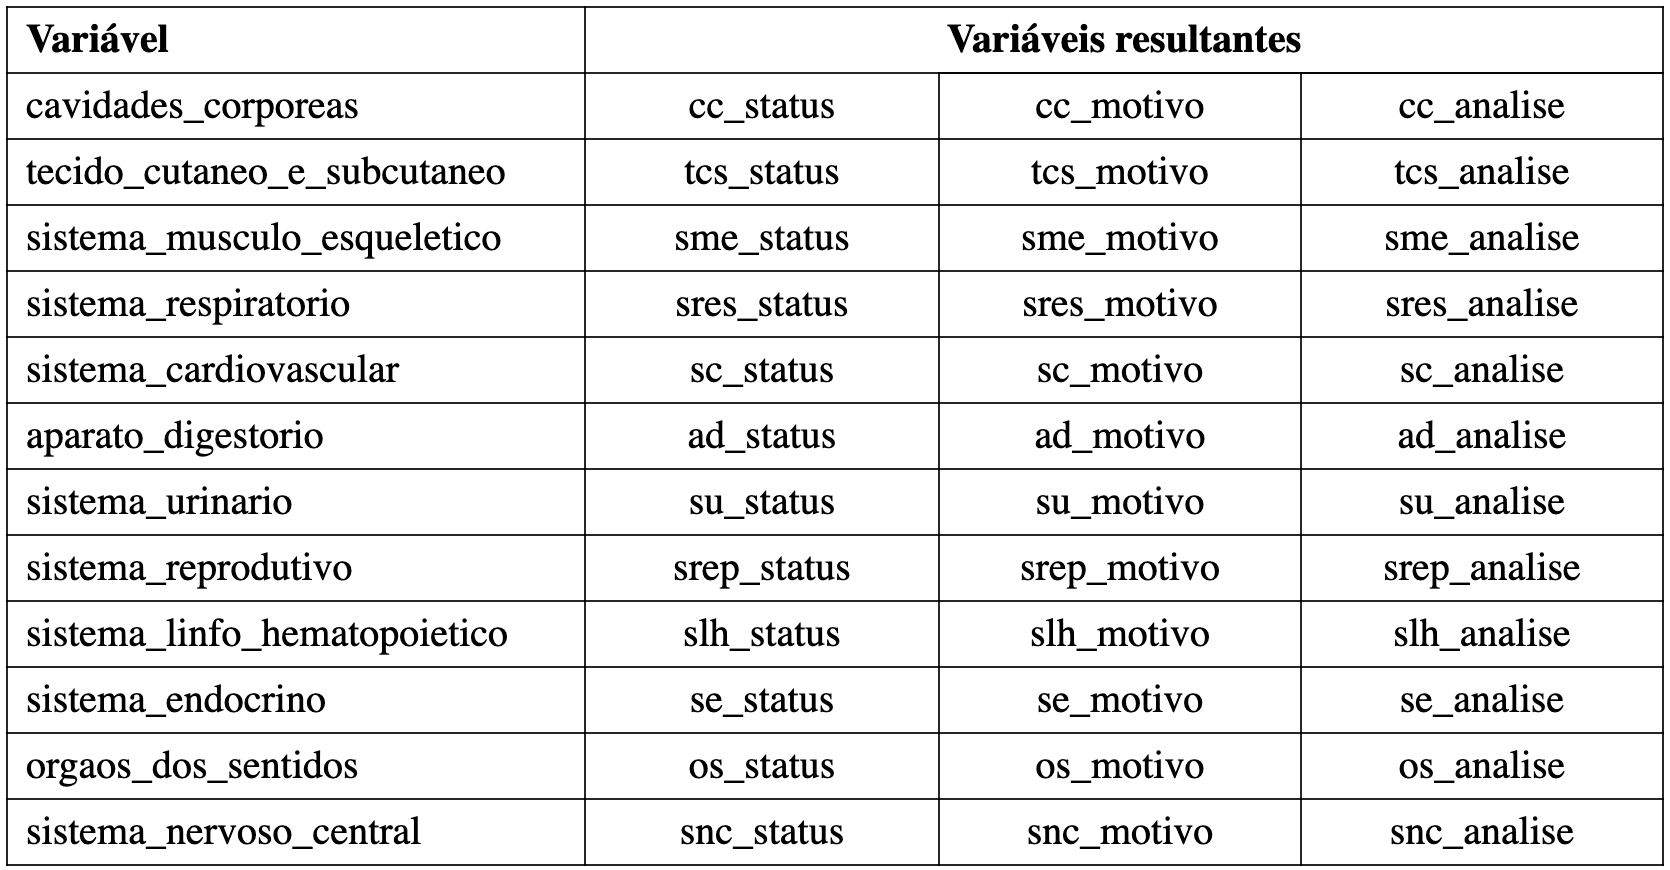
\includegraphics[width=.8\textwidth]{tabela_spread_variaveis.png}
\end{table}

\subsubsection{Variáveis Textuais}

Como a maioria dos dados é apresentado de forma textual, foram necessários alguns tratamentos para eliminar possíveis inconsistências entre registros. Todos os valores foram convertidos para letras minúsculas, removendo acentuações e pontuações.

Após a aplicação dos tratamentos ainda foi realizada a conversão das colunas identificadas como \textit{chr} para o tipo \textit{factor}. Assim, permitindo a verificação da correlação entre as variáveis a serem utilizadas no modelo.

\subsubsection{Variáveis com Dados Vazios ou Nulos}

Após estes tratamentos, foi observado que algumas variáveis apresentavam textos vazios. Sendo que, para as variáveis \say{diagnostico\_presuntivo\_lesao\_principal\_orgao}, \say{diagnostico\_presuntivo\_lesao\_principal\_causa}, \say{diagnostico\_primario\_lesao\_principal\_orgao}, \say{diagnostico\_primario\_lesao\_principal\_causa} e \say{presenca\_de\_residuos\_solidos} os dados vazios foram alterados para \say{indeterminado}, permitindo analisar alguns padrões importantes.  As demais variáveis foram convertidas para \textit{NA}.

Verificou-se, conforme demonstrado na figura \ref{fig:pre_missing_data}, o percentual de ausência de dados para cada variável que poderia ser utilizada no modelo. Optou-se por manter apenas as variáveis classificadas como \say{boas} na verificação de dados ausentes.

\begin{figure}[ht]
\centering
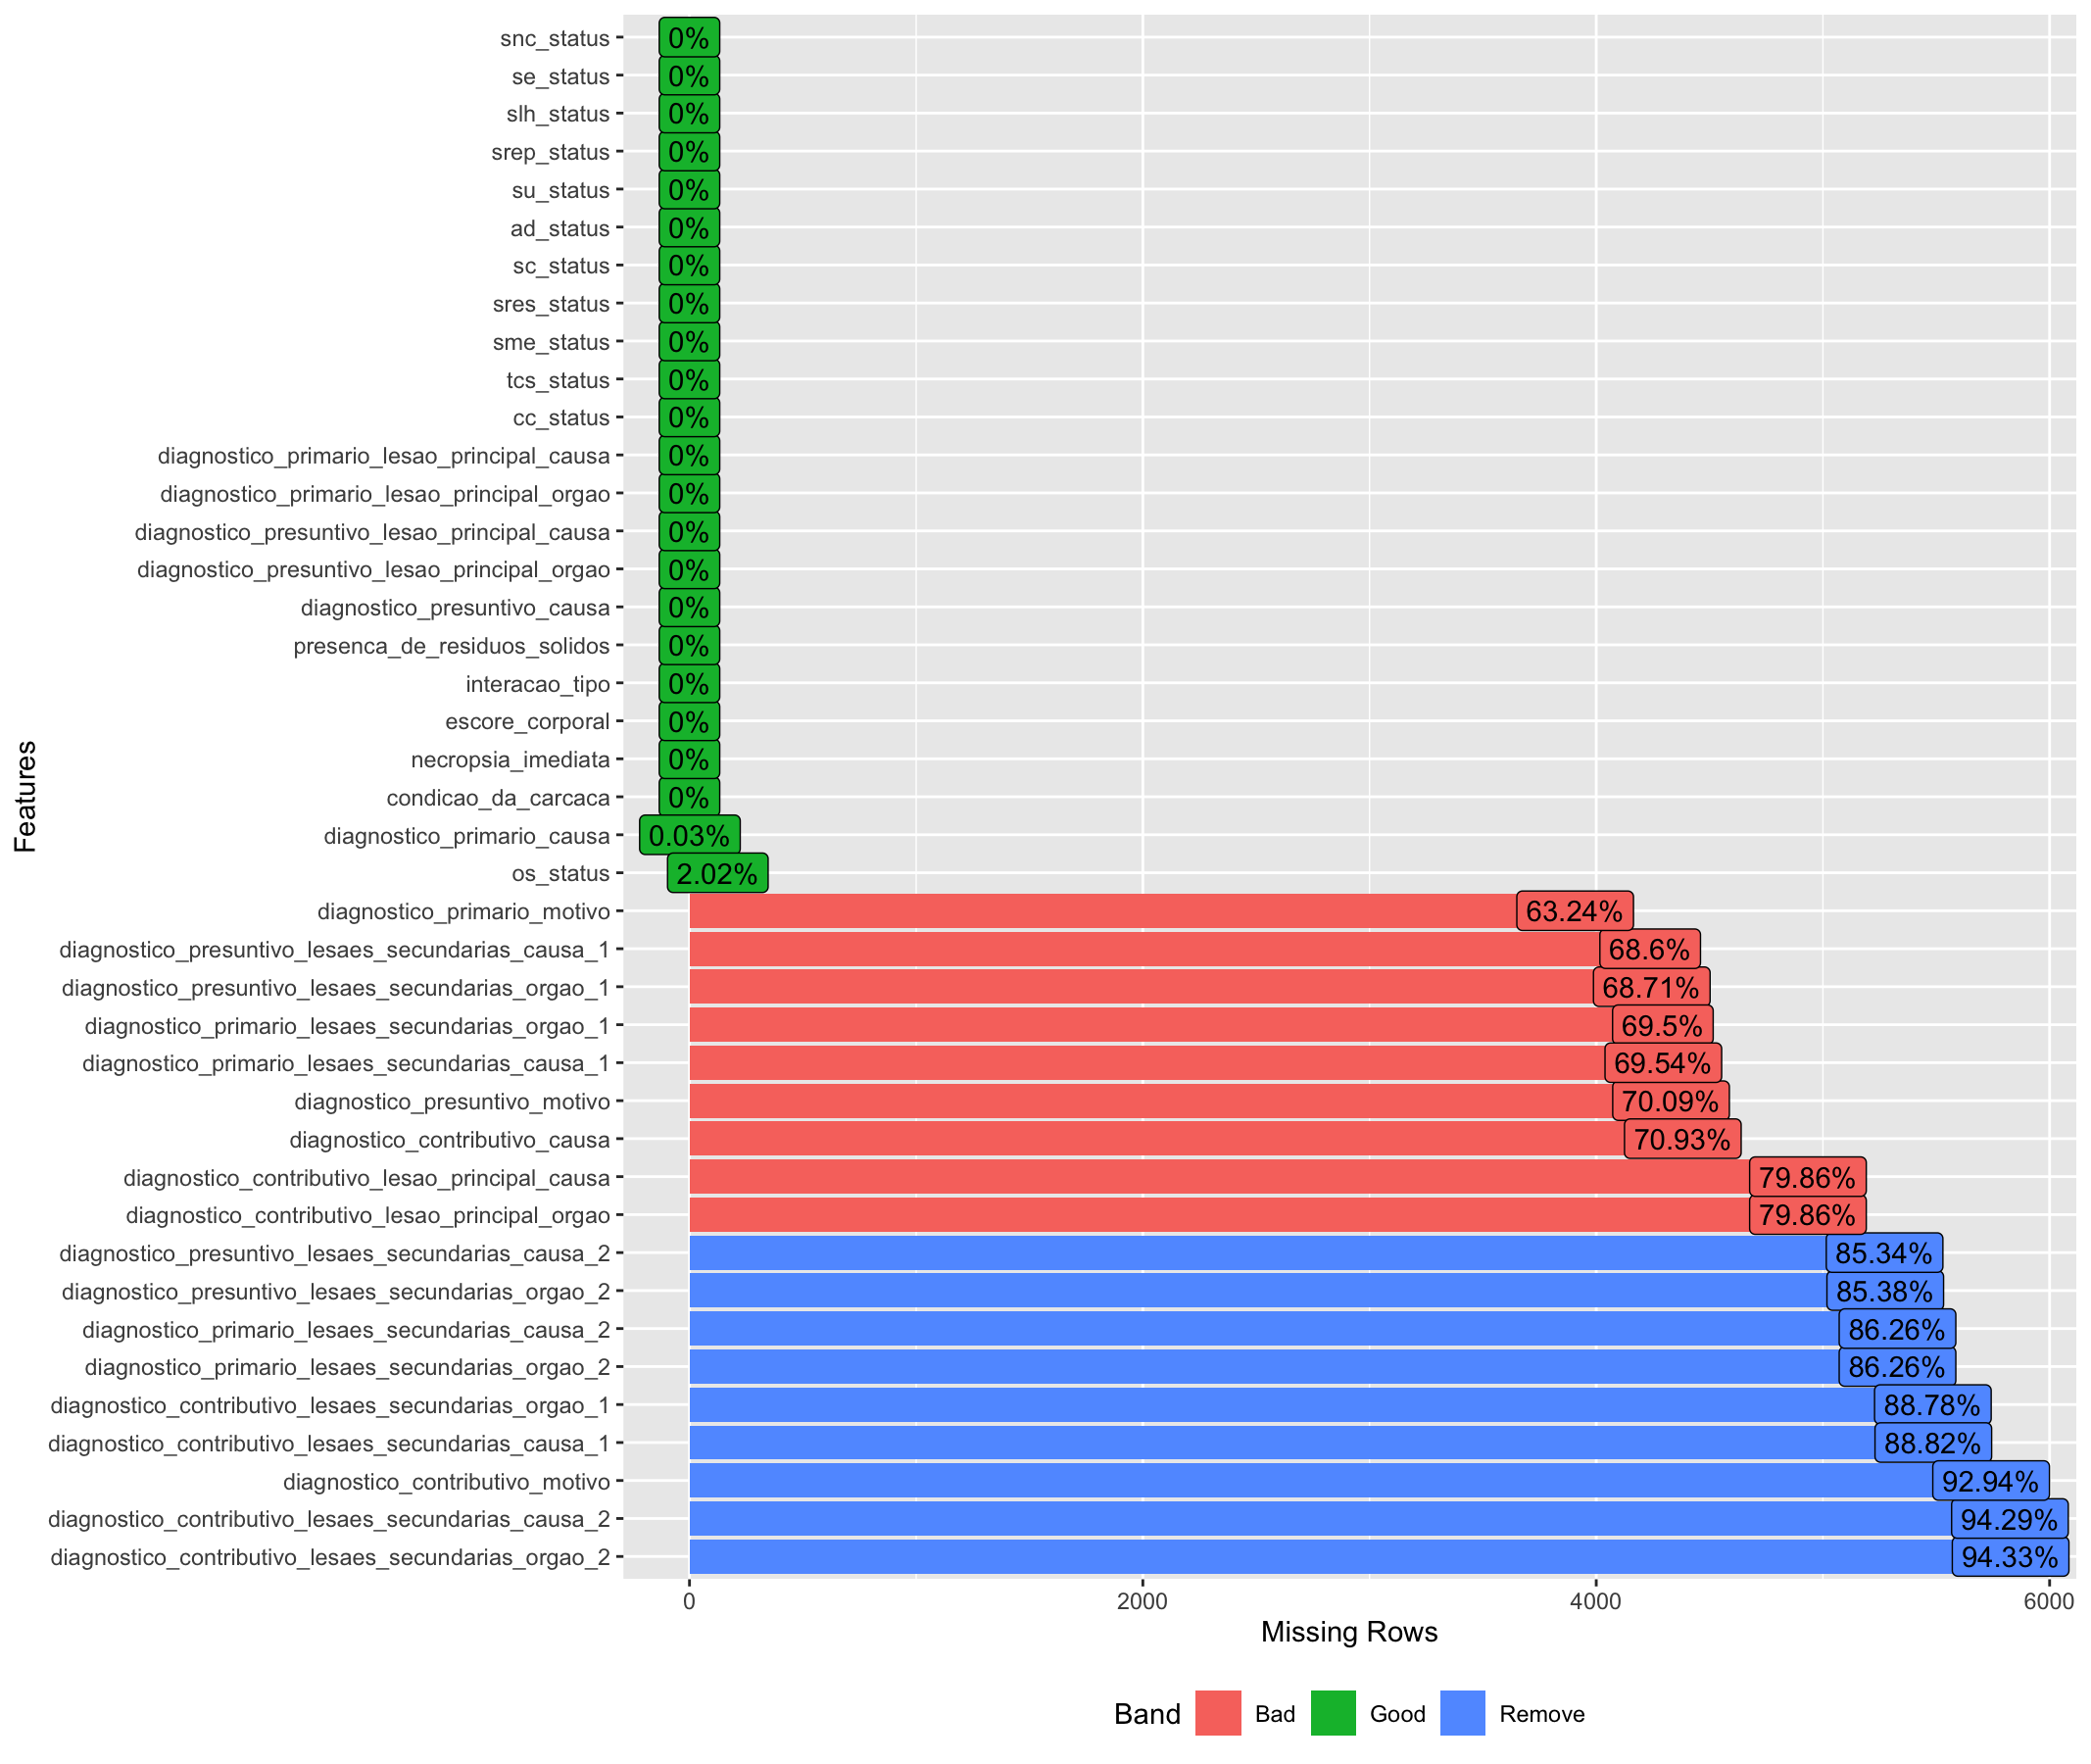
\includegraphics[width=.8\textwidth]{dados_faltantes_pre_limpeza.png}
\caption{Percentual de ausência de dados por variável}
\label{fig:pre_missing_data}
\end{figure}

\subsection{Pré Processamento}

- Enumerar pontos abordados nas subseções seguintes.

\subsubsection{Correlação}

A correlação entre duas variáveis refere-se ao Coeficiente de Correlação de Pearson e é um indicador que mede relação entre duas variáveis. A medida compreende um intervalo entre -1 e +1 sendo que, quanto mais próximo dos extremos, mais forte é a relação e, quanto mais próximo de zero, mais fraca é a relação \cite{lantz:mlinR}.

Correlações negativamente fortes implicam que, ao aumentar o valor de uma variável, a variável correlacionada terá seu valor diminuído. Já as correlações positivamente fortes implicam que, ao aumentar o valor de uma variável, sua correlacionada também aumentará \cite{lantz:mlinR, aggarwal:dcaa}.

Na figura \ref{fig:correlation} é possível observar a correlação entre as variáveis após o processo de limpeza da base. Pode-se perceber que existem algumas correlações relativamente fortes, principalmente nas variáveis referentes aos órgãos do animal.

\begin{figure}[ht]
\centering
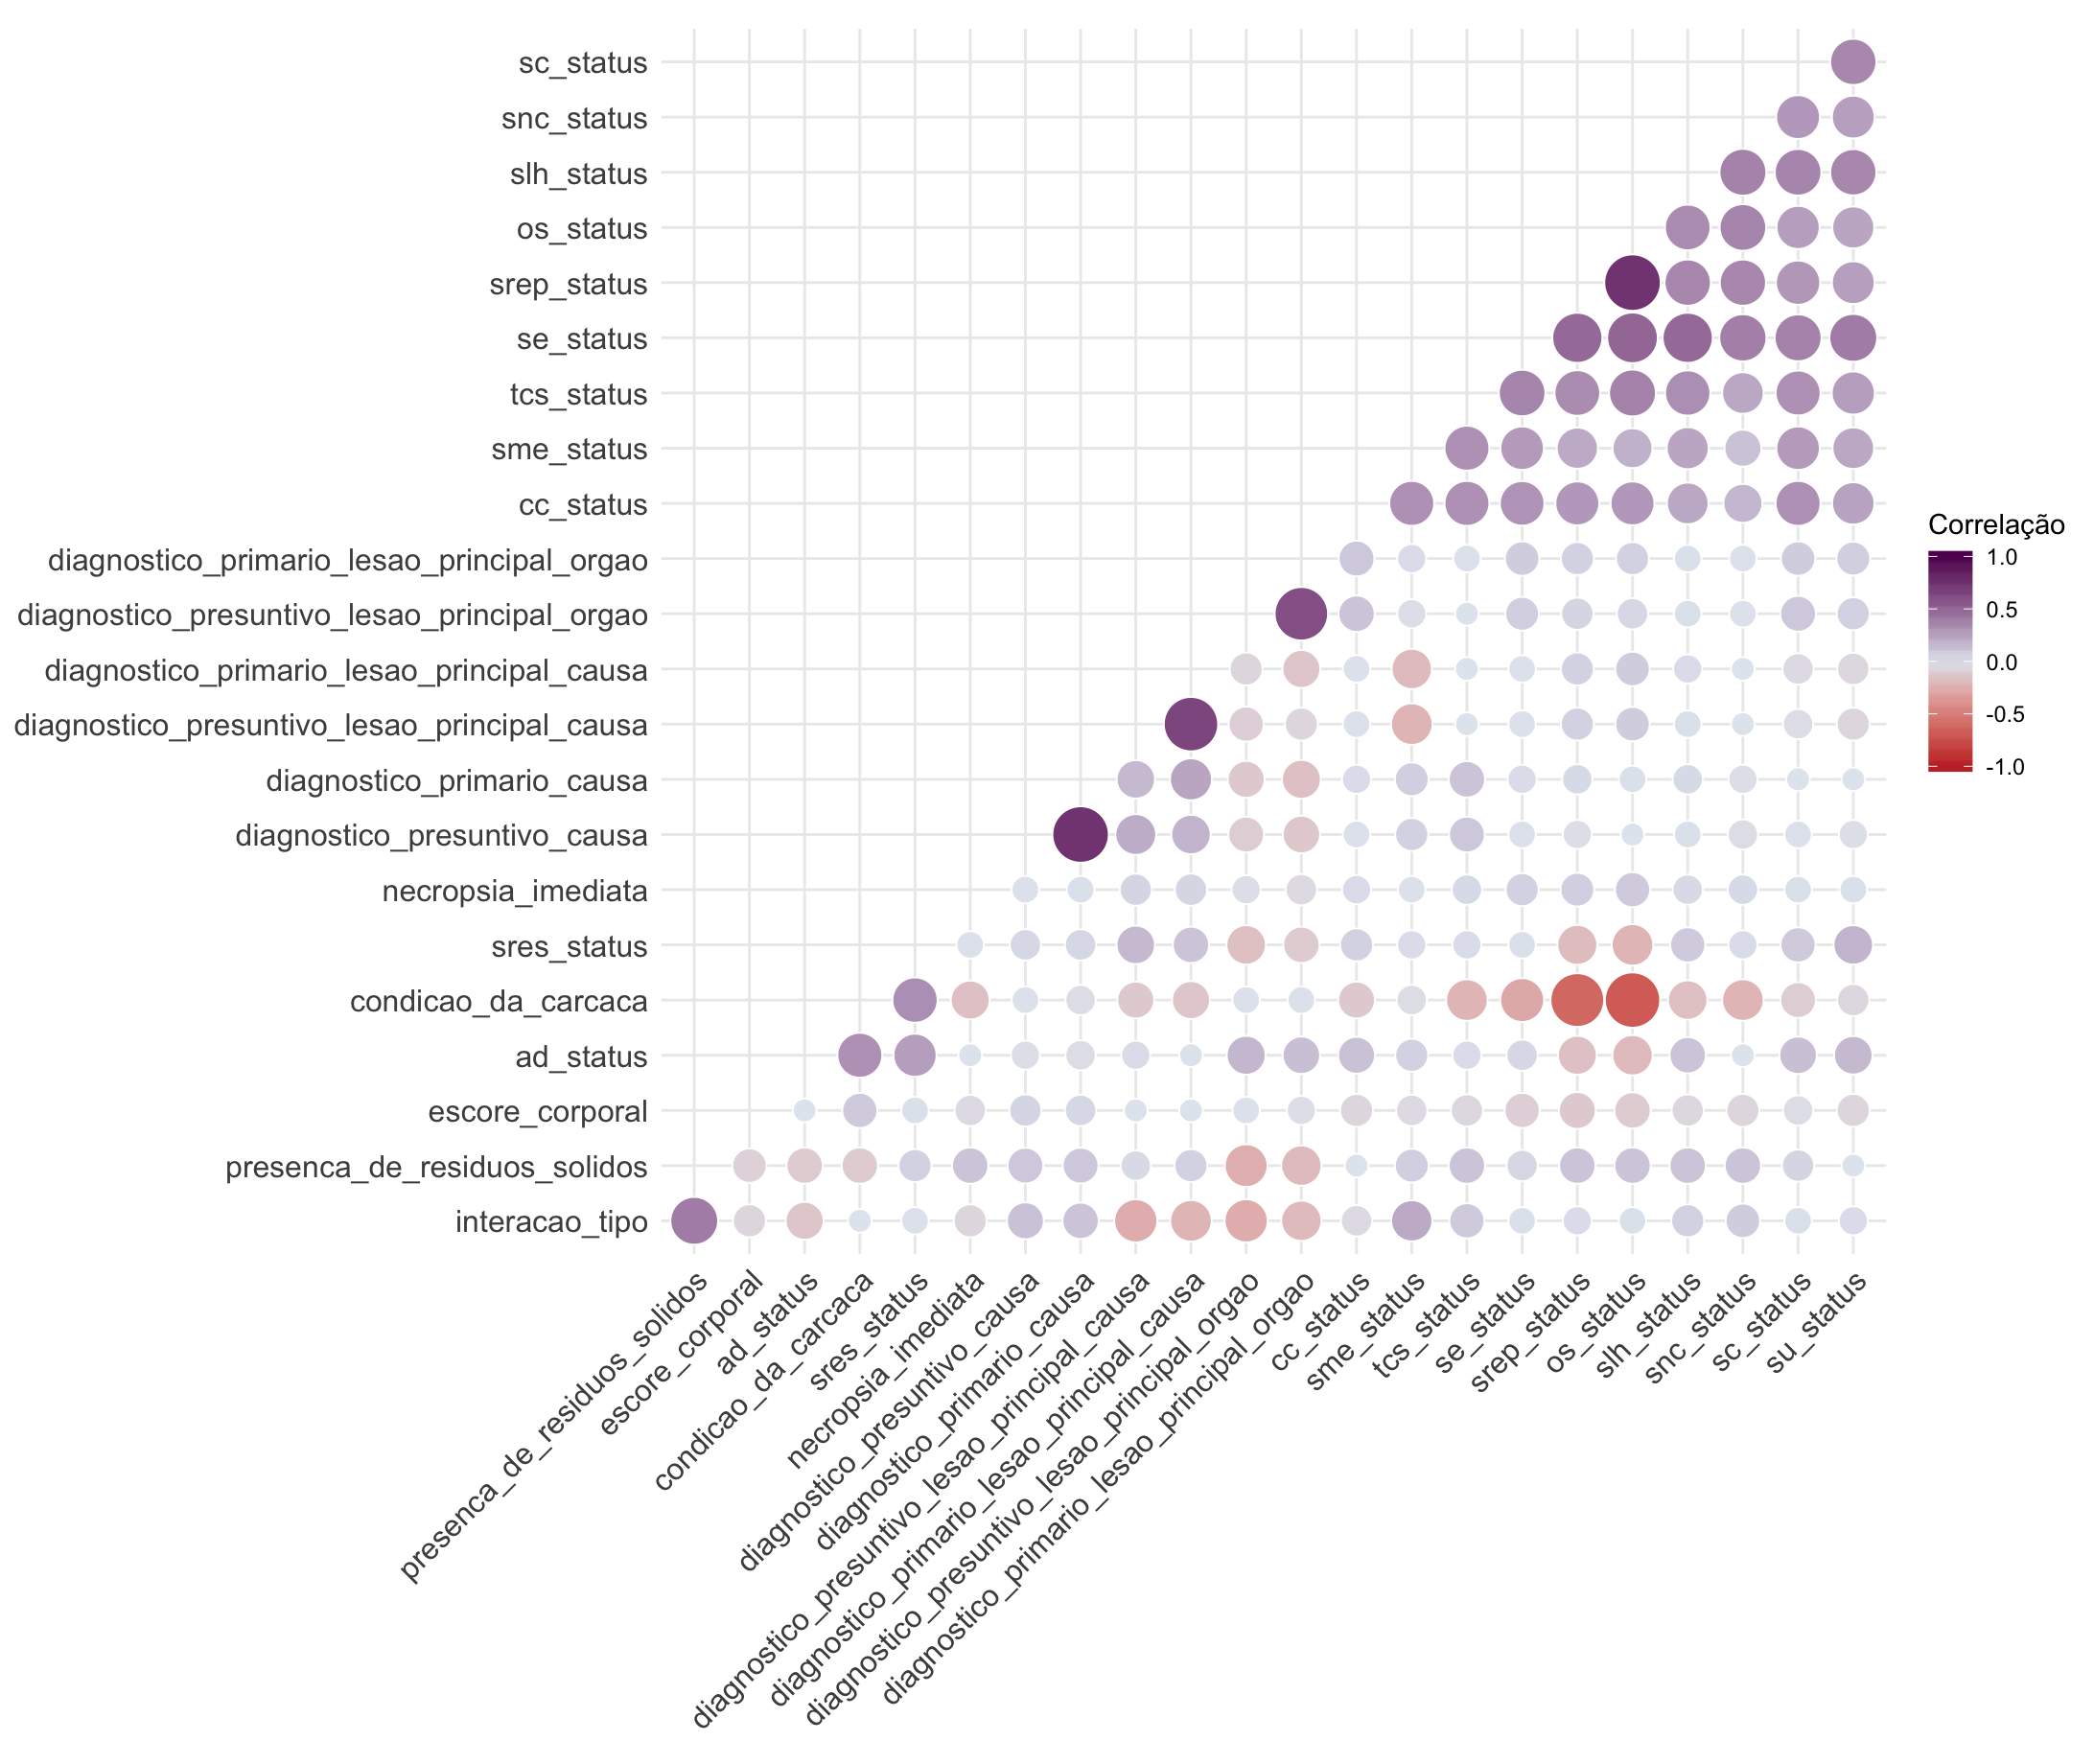
\includegraphics[width=.8\textwidth]{correlacao_dados_sem_na.png}
\caption{Correlação entre as variáveis}
\label{fig:correlation}
\end{figure}

\subsubsection{Separação dos Dados}

Por fim, para gerar os modelos classificadores, as variáveis utilizadas no modelo foram normalizadas utilizando a padronização \textit{z-score} com o objetivo de garantir que valores distoantes de cada variável tenham seu impacto considerado \cite{lantz:mlinR}.

Após a padronização dos valores, a base final foi divida em duas partes: (i) Base de treino, utilizada para construir e treinar os modelos; e (ii) Base de testes, a qual foi utilizada para medir a acurácia de cada modelo obtido. Esta divisão foi realizada a partir da seleção aleatória dos registros em uma proporção de 70\% do total de registros para a base de treino e 30\% para a base de teste.
    
\subsection{Processamento}

Para gerar os modelos de aprendizagem de máquina utilizou-se o pacote \textit{caret} da linguagem R, o qual fornece diversas funcionalidades desde o momento de divisão dos dados até estimativa de importância de cada variável para o modelo \cite{caret:r}.

Todos os algoritmos testados nesta pesquisa foram treinados utilizando o método \textit{cross-validation} (CV), o qual consiste em dividir os dados de treino em \textit{n} conjuntos menores. Um dos \textit{n} conjuntos é utilizado para treinar o modelo enquanto os outros \textit{n-1} conjuntos são utilizados para teste \cite{lantz:mlinR}. 

O CV foi parametrizado para repetir este processo 10 vezes utilizando 10 subconjuntos em cada processo.

\subsubsection{Naive Bayes}

\textit{Naive Bayes (NB)} é um algoritmo de classificação que faz uso do teorema de Bayes. É um algoritmo simples, mas que se tornou bastante utilizado, principalmente na classificação de textos. Possui este nome pelo fato de realizar suposições \textit{ingênuas} sobre os dados. Este algoritmo assume que todas as variáveis da base são igualmente importantes e independentes, por exemplo \cite{lantz:mlinR, aggarwal:dcaa}.

Apesar de ser simples e funcionar bem com dados distoantes, ainda depende de suposições fracas em relação às variáveis e não é ideal em bases com um número muito grande de variáveis numéricas \cite{lantz:mlinR}.

O pacote \textit{caret} fornece o método \textit{naive\_bayes} que aceita três parâmetros de ajuste do modelo, sendo: (i) \textit{laplace}, utilizado para aplicar a correção de Laplace, a qual serve para evitar que a probabilidade de um evento acontecer seja nula \cite{lantz:mlinR, caret:r}; (ii) \textit{usekernel}, permite alterar o modelo de estimativa de densidade para variáveis contínuas; e (iii) \textit{adjust}, permite ajustar a flexibilidade da estimativa de densidade do kernel.

A parametrização foi realizada com a opção \textit{usekernel} sempre \textit{TRUE} para garantir uma melhor estimativa dos dados numéricos da tabela. Foram testadas opções com \textit{laplace} entre 0 e 1 para \textit{adjust} entre 1 - 3. Conforme pode ser observado na figura \ref{fig:nb_resultados} o aumento da flexibilidade do kernel diminuiu a acurácia do modelo. Também é possível observar que o melhor resultado obtido foi utilizando \textit{laplace = 0} e \textit{adjsut = 1}, atingindo uma acurácia de 69,03\%. Ao aplicar o modelo na base de testes a acurácia atingiu 70,14\%.

\begin{figure}[ht]
\centering
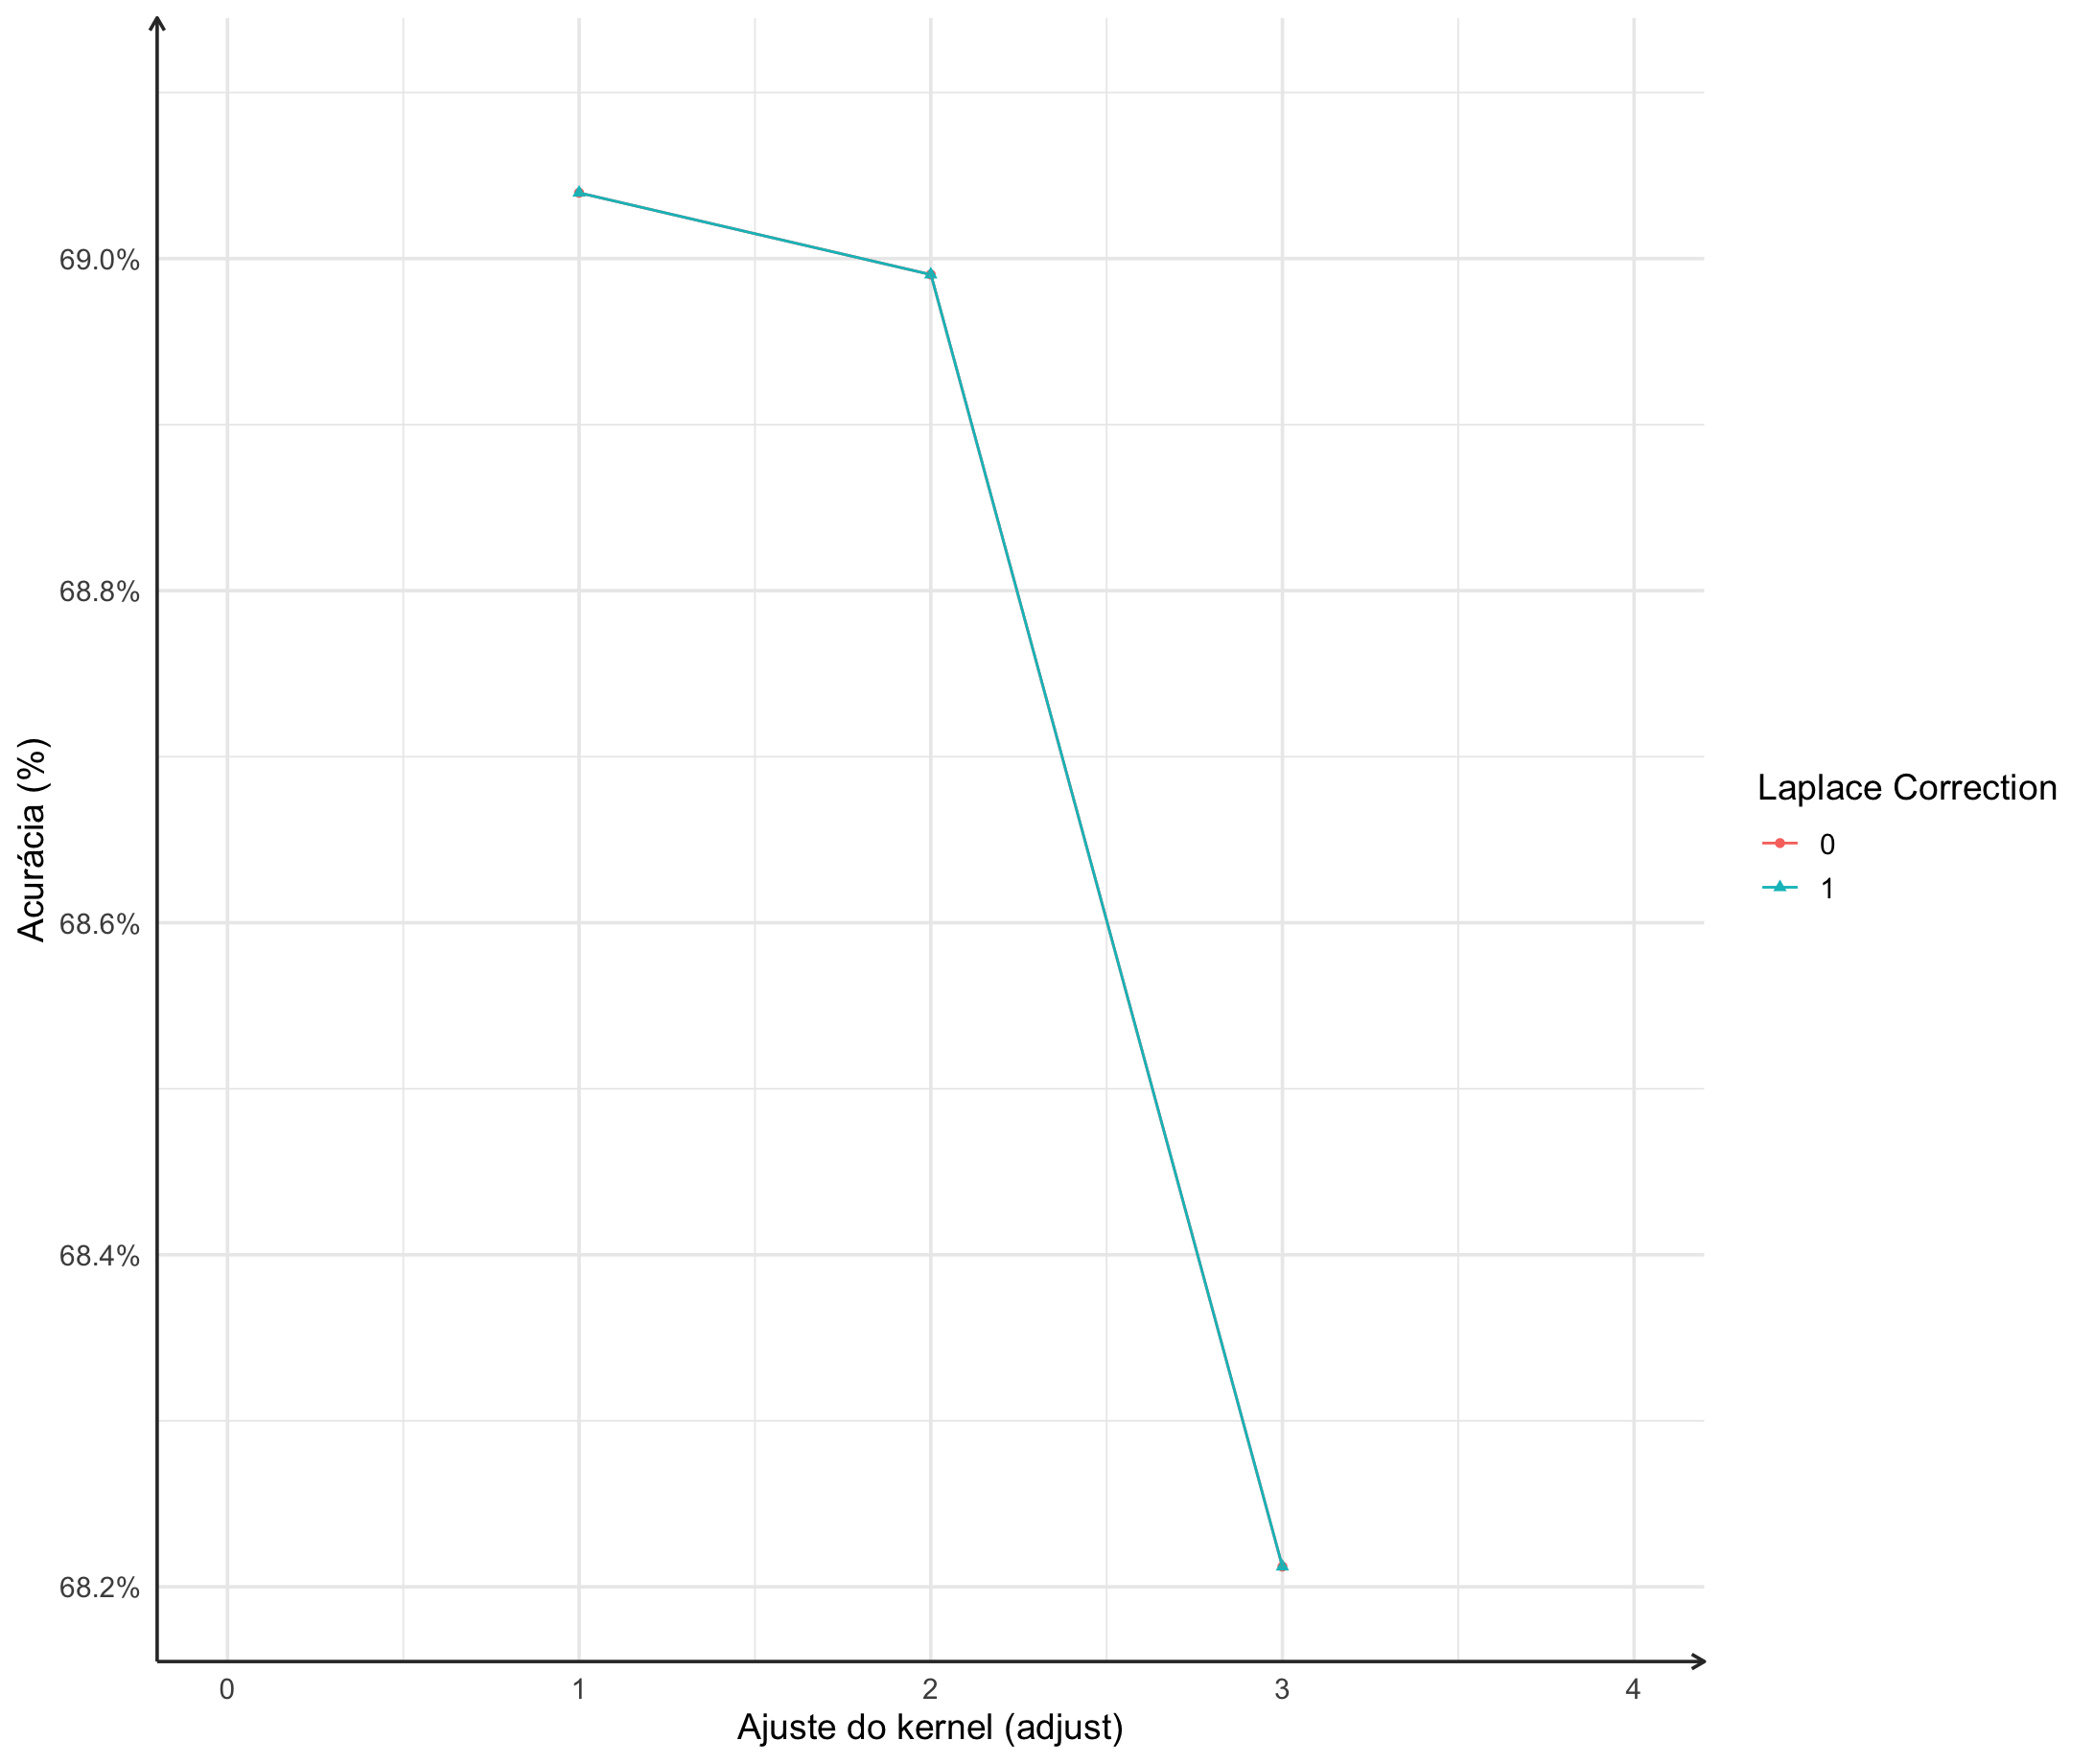
\includegraphics[width=.8\textwidth]{nb_resultados.png}
\caption{Resultados da parametrização para o modelo NB}
\label{fig:nb_resultados}
\end{figure}

\subsubsection{k-Nearest Neighbor}

O algoritmo de classificação \textit{k-Nearest Neighbor (kNN)} busca por \textit{k} registros similares ao registro sendo testado e assume a classe de maior ocorrência dentro dos similares encontrados. Para selecionar os registros similares o algoritmo calcula a distância entre os registros comparando os valores de cada variável do registro  \cite{lantz:mlinR}.

A escolha do valor de \textit{k} é importante para garantir que o modelo não vá sofrer com variações causadas por ruídos nos dados nem ignorar padrões importantes. Geralmente é utilizado um valor entre 3 e 10. Outra prática comum é utilizar um valor que seja a raíz quadrada do total de registros de treino \cite{lantz:mlinR, bonaccorso:mla}.

O pacote \textit{caret} fornece o método \textit{knn} que aceita como parâmetro apenas o valor de \textit{k}. A parametrização foi realizada com valores de \textit{k} entre 5 e 43 e, conforme pode ser observado na figura \ref{fig:knn_resultados}, a melhor acurácia obtida foi de 74,36\% utilizando um valor de \textit{k = 9}. Ainda é interessante verificar que o aumento dos valores de \textit{k} não auxiliou na performance do modelo. Ao aplicar o modelo na base de testes a acurácia atingiu 75,33\%.

\begin{figure}[ht]
\centering
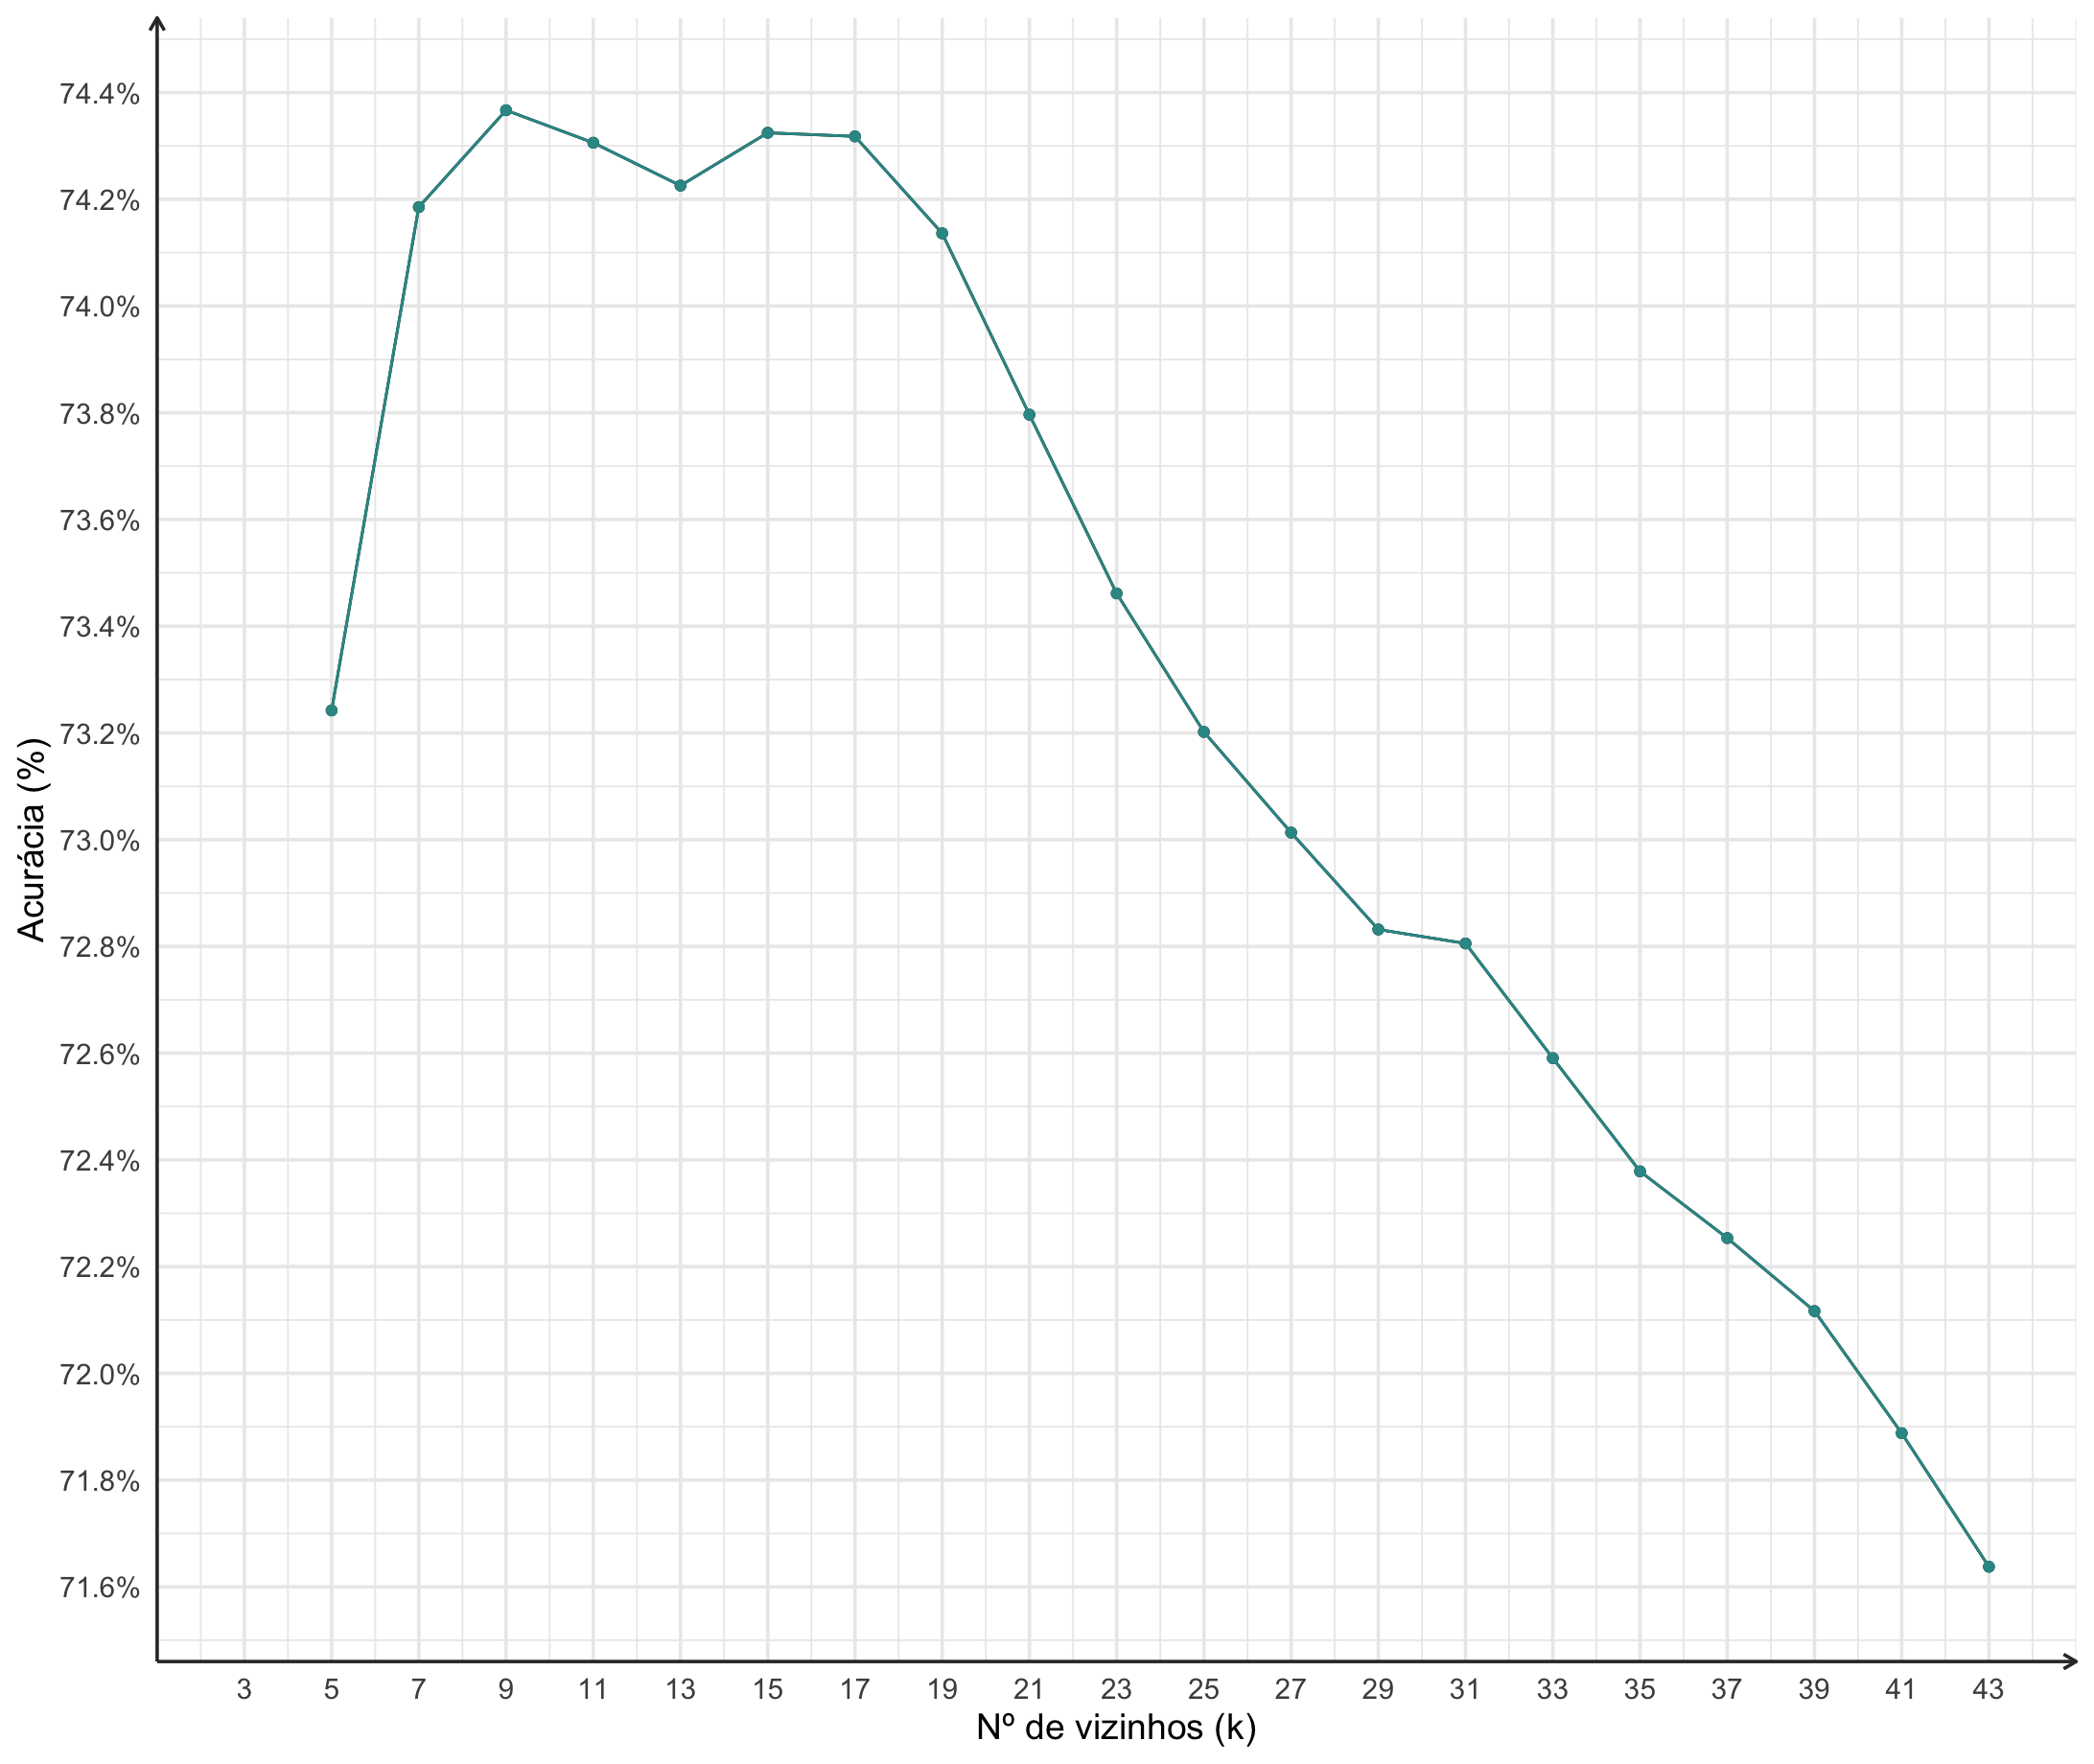
\includegraphics[width=.8\textwidth]{knn_resultados.png}
\caption{Resultados da parametrização para o modelo kNN}
\label{fig:knn_resultados}
\end{figure}

\subsubsection{Decision Tree}

Algoritmos de \textit{Decision Tree (DT)} utilizam um modelo semelhante a uma árvore, onde as ramificações representam observações e/ou decisões tomadas para chegar a uma conclusão/objetivo (extremidades ou folhas) \cite{lantz:mlinR, aggarwal:dcaa}.

No \textit{caret} é possível escolher entre diversas implementações de algoritmos de árvores. Dentre as opções adequadas, optou-se por utilizar um dos modelos mais conceituados, o qual foi desenvolvido pelo cientista da computação J. Ross Quinlan, denominado C5.0 \cite{lantz:mlinR, caret:r}.

A implementação fornecida pelo pacote \textit{caret} oferece a possibilidade de customizar três parâmetros, sendo: (i) \textit{trials}, indica o máximo de árvores paralelas utilizadas para selecionar a melhor classificação; (ii) \textit{model}, indica se o modelo deve utilizar árvore ou decompor a estrutura para um conjunto de regras; e (iii) \textit{winnow}, utilizado para indicar se o modelo deve pré selecionar as variáveis de maior impacto \cite{caret:r, cran:r}. 


Para a parametrização  do modelo nesta pesquisa utilizou-se: valores de 1 a 15 para \textit{trial}, \textit{\say{rules}} ou \textit{\say{tree}} para \textit{model} e \textit{TRUE} ou \textit{FALSE} para \textit{winnow}.  Ressalta-se que todas as combinações possíveis destes valores foram executadas e testadas. A figura \ref{fig:dt_resultados} apresenta os resultados dos modelos obtidos para todas as combinações exploradas.

Observa-se que, ao pré selecionar variáveis de maior impacto, a performance do modelo foi prejudicada, uma vez que seus resultados são inferiores em comparação aos resultados sem pré seleção. Como há um conjunto considerável de variáveis, é possível que o processo tenha desconsiderado pequenos detalhes causando um efeito indesejado no resultado final.

Também pode-se observar que o resultado mais expressivo foi alcançado utilizando \textit{model = 'rules'} e \textit{trials = 13}. Com esta parametrização o modelo conseguiu uma acurácia de 78.29\%. Ao aplicar o modelo na base de testes a acurácia atingiu 78.92\%.

\begin{figure}[ht]
\centering
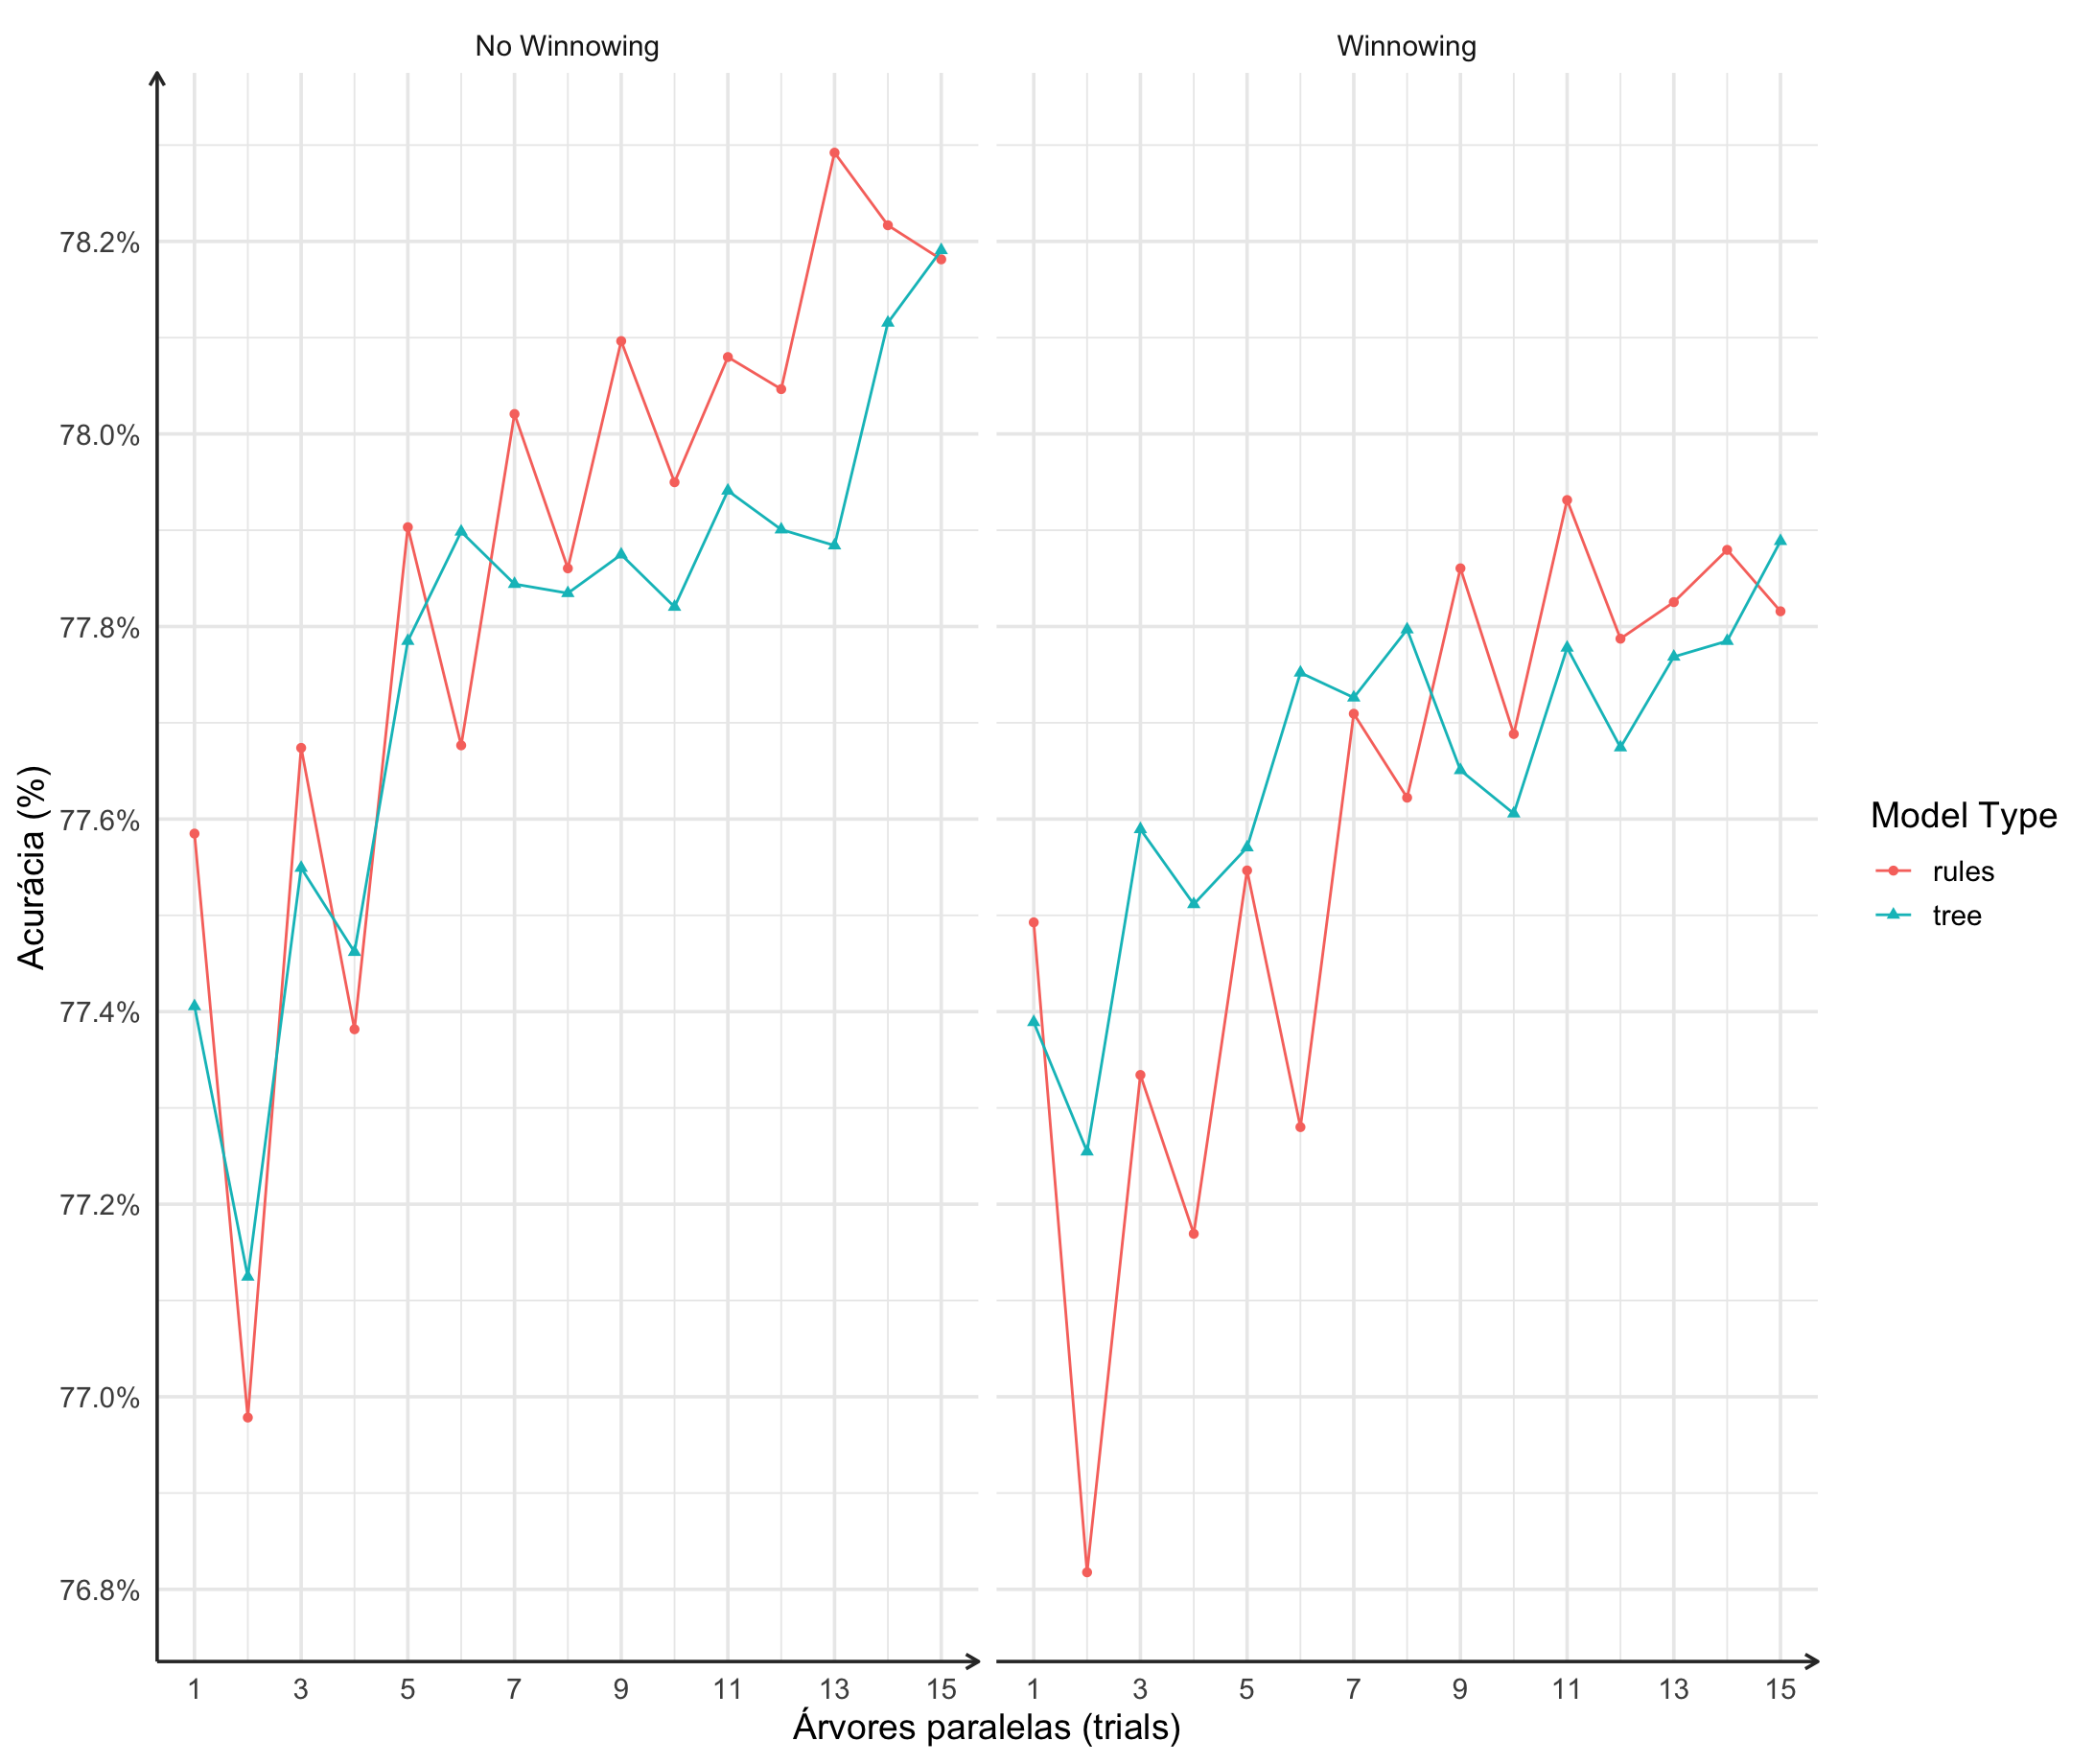
\includegraphics[width=.8\textwidth]{dt_resultados.png}
\caption{Resultados da parametrização para o modelo DT}
\label{fig:dt_resultados}
\end{figure}

\subsubsection{Random Forest}

\textit{Random Forest (RF)} é um método baseado em conjuntos de DT e foi definido por Leo Breiman e Adele Cutler. Este modelo trabalha com uma seleção alteatória de variáveis para diversificar os modelos de DT. O algoritmo gera um conjunto de árvores de decisão e combina suas predições, resultando em um modelo bastante funcional para a maioria dos problemas \cite{lantz:mlinR, breiman:rf}.

Existem algumas boas implementações de RF no pacote \textit{caret}. Dentre as mais adequadas, optou-se por utilizar o método \textit{ranger}, o qual se mostrou bastante rápido e eficiente, mesmo lidando com grandes volumes de dados \cite{ranger:rf, caret:r}.

Ao utilizar esta implementação é possível customizar três parâmetros para melhorar a performance do modelo, sendo: (i) \textit{mtry}, que indica a quantidade de variáveis a serem selecionadas aleatoriamente; (ii) \textit{splitrule}, indica o algoritmo utilizado para realizar as divisões de árvore; e (iii) \textit{min.node.size} controla a complexidade das árvores, onde valores baixos garantem árvores mais complexas  enquanto valores maiores geram árvores com pouca complexidade .

É importante considerar que árvores de alta complexidade aumentam o risco de padrões específicos demais para o conjunto de dados de treino (\textit{overfitting}). Enquanto árvores pouco complexas podem não perceberm alguns padrões importantes, deixando o modelo muito flexível (\textit{underfitting}).

Para encontrar o melhor modelo, foram testados diversos conjuntos de parâmetros. Foram utilizadas \textit{2, 4, 8, 16 ou 20} variáveis selecionadas aleatoriamente, combinadas com \textit{'gini', 'extratrees'} para \textit{splitrule} e o \textit{min.node.size} sendo \textit{1, 3 ou 5}. A figura \ref{fig:rf_resultados} apresenta um comparativo para os modelos obtidos. Observa-se que a utilização de muitas variáveis acaba prejudicando a performance do modelo, indicando que utilizar todas as variáveis diretamente não é uma boa prática. 

O melhor modelo obtido teve os seguintes parâmetros: \textit{mtry = 4}, \textit{splitrule = 'gini'} e \textit{min.node.size = 5} e obteve uma acurácia de 78.63\%. Ao aplicar o modelo na base de testes a acurácia atingiu 79.75\%.

\begin{figure}[ht]
\centering
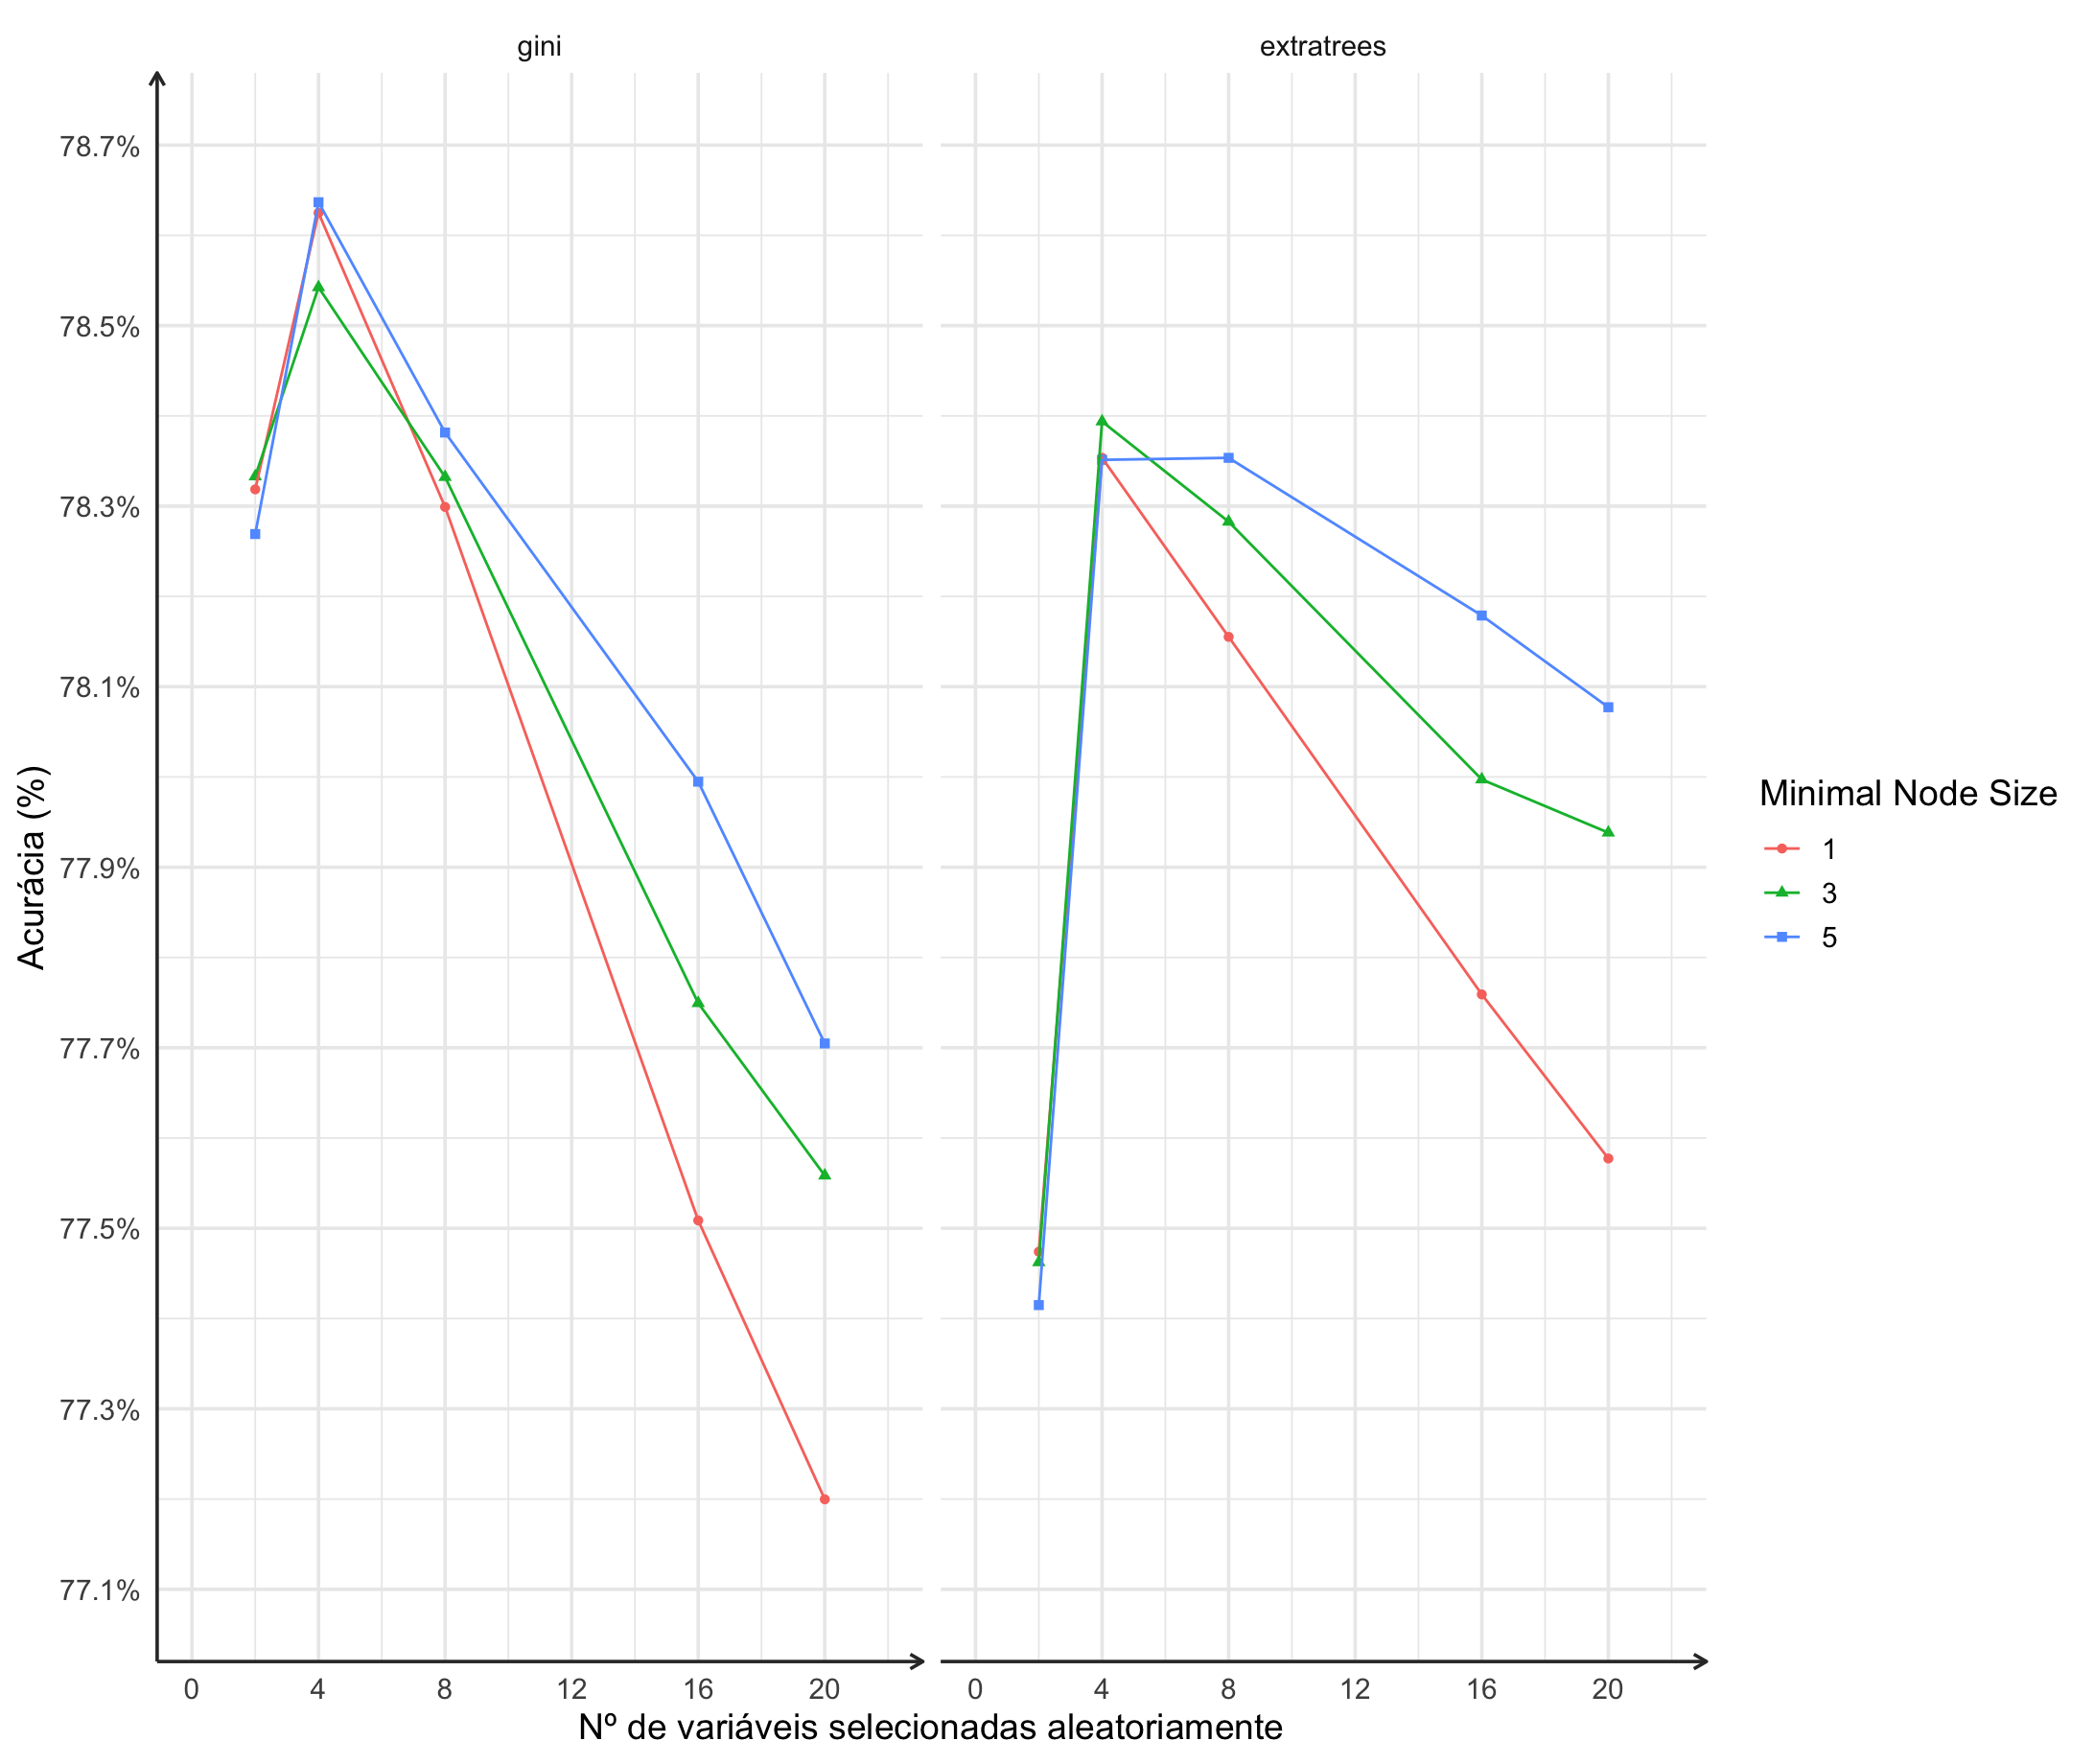
\includegraphics[width=.8\textwidth]{rf_resultados.png}
\caption{Resultados da parametrização para o modelo RF}
\label{fig:rf_resultados}
\end{figure}

\section{Conclusão}

Após o processo de análise, limpeza e processamento dos algoritmos de aprendizagem de máquina, foi possível obter modelos com um percentual de acurácia suficientemente aceitável para uma primeira abordagem nos dados de necropsia. Os modelos de RF e DT obtiveram resultados bastante próximos. Com uma acurácia de pouco mais de 79\%, o RF foi capaz predizer se houve alguma interação de influência do ser humano e os animais necropsiados pelo PMP-BS.

Ainda sobre os modelos obtidos, é importante salientar que todos tiveram maior capacidade de identificar corretamente verdadeiros negativos (especificidade). A capacidade de identificar corretamente verdadeiros positivos (sensibilidade) teve bastante oscilação dependendo da classe em questão, sendo que os modelos foram mais capazes de inferir as classes \say{interação com lixo} e \say{interação com pesca}.

O processo de compreensão e limpeza dos dados obtidos foi bastante oneroso, consumindo cerca de 80\% de todo o processo da pesquisa. É importante compreender a importância de cada informação e quais os impactos que as variáveis podem causar na obtenção dos modelos. A remoção ou o uso exagerado de variáveis pode deixar o modelo tendencioso. O que impede o mesmo de detectar padrões, impactando negativamente na performance.

Ainda em relação à limpeza dos dados, a qualidade dos registros teve bastante impacto na análise. Diversas variáveis possuíam preenchimento fora do padrão ou nulos, enquanto outras possuíam mais de um tipo de informação. Seria interessante, talvez, uma melhor organização das informações, prevenindo inconsistências nos dados de entrada sem restrição de preenchimento.

Finalizando, apesar dos bons resultados obtidos em uma primeira pesquisa e exploração de possíveis modelos para identificar interações antrópicas em animais coletados nas regiões costeiras, fica clara a possibilidade de continuação e aperfeiçoamento das análise e modelos obtidos.

Uma possível continuação da pesquisa envolve considerar, também, as necropsias que possuam mais de uma interação antrópica ao mesmo tempo, identificando outros padrões não percebidos nesta pesquisa. Também é possível analisar variáveis textuais para extrair características que possam ser relevantes ao contexto da análise por parte do modelo.

\bibliographystyle{sbc}
\bibliography{referencias}

\end{document}
